% Figure 3: Buddy IPAM - controller and per-node agent
% Same drawing as in ppt/project2/slides.tex. Compile: pdflatex fig3_ipam_architecture.tex
\documentclass[border=4pt]{standalone}
\usepackage{amssymb}
\usepackage{tikz}
\usetikzlibrary{arrows.meta, positioning, fit, backgrounds, calc}
\renewcommand{\familydefault}{\sfdefault}
\tikzset{
  box/.style={draw, rounded corners, align=center, font=\scriptsize,
    minimum width=2.4cm, minimum height=0.6cm},
  arr/.style={-{Stealth[length=1.6mm]}, thick},
  biarr/.style={{Stealth[length=1.6mm]}-{Stealth[length=1.6mm]}, thick},
}
\begin{document}
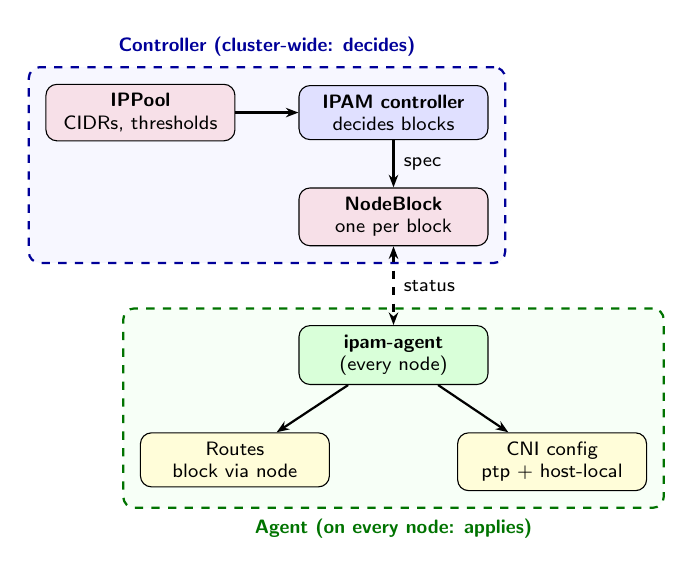
\begin{tikzpicture}
  \node[box, fill=purple!12] (pool) {\textbf{IPPool}\\CIDRs, thresholds};
  \node[box, fill=blue!12, right=0.8cm of pool] (ctrl) {\textbf{IPAM controller}\\decides blocks};
  \node[box, fill=purple!12, below=0.6cm of ctrl] (nb) {\textbf{NodeBlock}\\one per block};
  \node[box, fill=green!15, below=1.0cm of nb] (ag) {\textbf{ipam-agent}\\(every node)};
  \node[box, fill=yellow!15, below left=0.6cm and -0.4cm of ag] (rt) {Routes\\block via node};
  \node[box, fill=yellow!15, below right=0.6cm and -0.4cm of ag] (cfg) {CNI config\\ptp + host-local};
  \draw[arr] (pool) -- (ctrl);
  \draw[arr] (ctrl) -- node[right, font=\scriptsize]{spec} (nb);
  \draw[biarr, dashed] (nb) -- node[right, font=\scriptsize]{status} (ag);
  \draw[arr] (ag) -- (rt);
  \draw[arr] (ag) -- (cfg);
  \begin{scope}[on background layer]
    \node[draw=blue!60!black, thick, dashed, rounded corners, fill=blue!3, fit=(pool)(ctrl)(nb), inner sep=6pt,
      label={[font=\scriptsize\bfseries, text=blue!60!black]north:Controller (cluster-wide: decides)}] {};
    \node[draw=green!45!black, thick, dashed, rounded corners, fill=green!3, fit=(ag)(rt)(cfg), inner sep=6pt,
      label={[font=\scriptsize\bfseries, text=green!45!black]south:Agent (on every node: applies)}] {};
  \end{scope}
\end{tikzpicture}
\end{document}
